% !TEX root =  ../supplementary.tex
\section{Personalized Biopsies Based on Risk of GS7}
\begin{figure}
\centerline{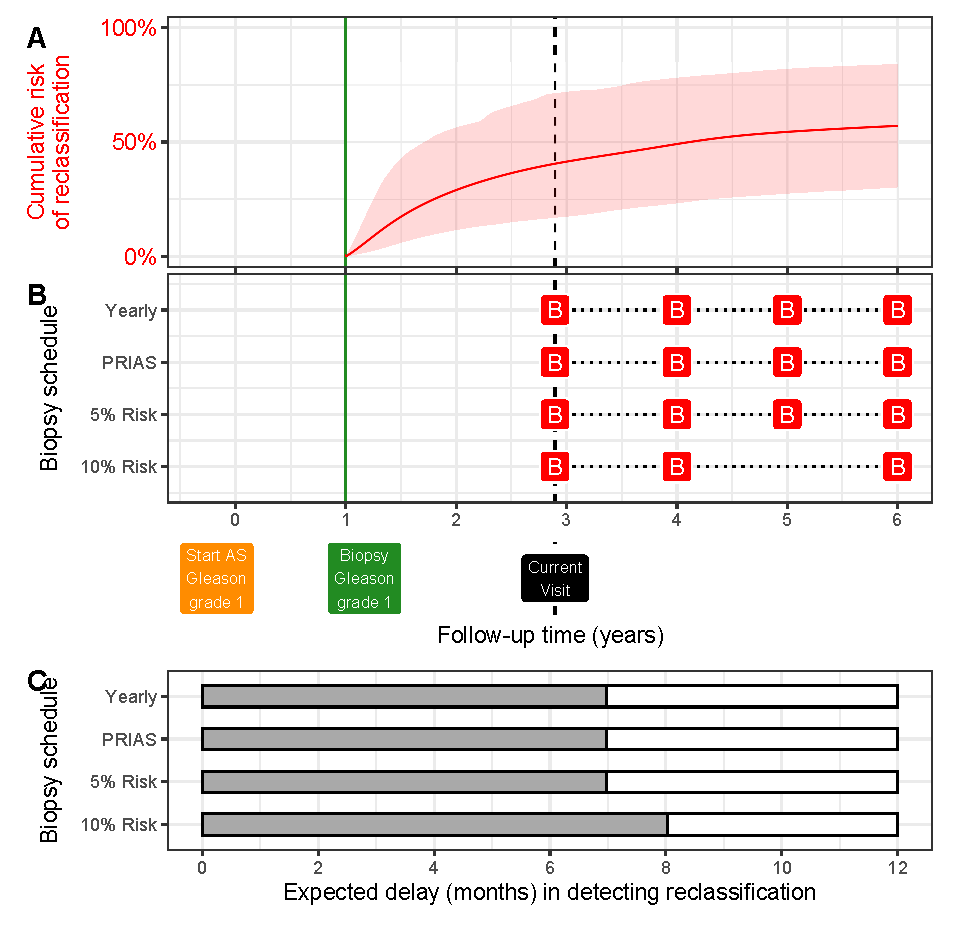
\includegraphics[width=\columnwidth]{images/demo_pat1.eps}}
\caption{\textbf{Illustration of the joint model fitted to the PRIAS dataset}. \textbf{Panel~A:} shows the observed and fitted $\log_2(\mbox{PSA} + 1)$ measurements (Equation~\ref{eq:long_model_psa}). \textbf{Panel~B:} shows the estimated $\log_2(\mbox{PSA} + 1)$ velocity (velocity cannot be observed directly) over time. The hazard function (Equation~\ref{eq:rel_risk_model}) shown in \textbf{Panel~C}, depends on the fitted $\log_2(\mbox{PSA} + 1)$ value and velocity.}
\label{fig:dynRiskPlot_2340}
\end{figure}